\section{Zielsetzung}
\label{sec:Ziel}
Im folgenden Versuch sollen die diskreten Energiewerte der Elektronenhülle des Hg-Atoms untersucht werden. Dazu wird die integrale Energieverteilung
der beschleunigten Elektronen bei zwei unterschiedlichen Temperaturen untersucht. Anschließend werden für zwei weitere Temperaturen Franck-Hertz-Kurven aufgenommen.

\section{Theorie}
\label{sec:Theorie}

\noindent
Zur Strukturauflkärung der Elektronenhüllen werden Elektronenstoßexperimente durchgeführt. Dazu werden Elektronen, die eine geeignete Energie haben, auf Atome geschossen. Es wird
der dabei entstehende Energieverlust der Elektronen dazu genutzt, Informationen über die Struktur zu erhalten.

\subsection{Aufbau und Ablauf des Franck-Hertz Experimentes}
\label{subsec:aufbau}
Die Franck-Hertz Apparatur ist schematisch in der \autoref{fig:franckAufb} dargestellt.

\begin{figure}[H]
    \centering
    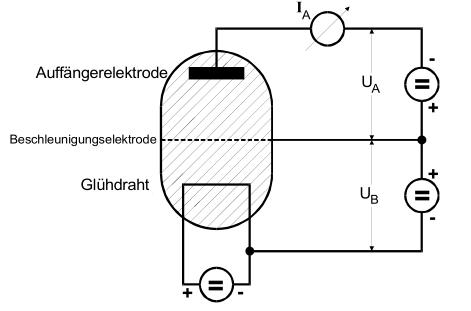
\includegraphics[width=0.75\textwidth]{data/FranckHertz.png}
    \caption{Schematische Darstellung des Franck-Hertz Versuches.}
    \label{fig:franckAufb}
\end{figure}

\noindent
Der Versuch besteht aus einem evakuierten Gefäß, in dem sich die auf die Struktur der Elektronenhülle zu untersuchende Probe befindet. In dem folgenden Versuch wird Quecksilber verwendet.
In der Glasglocke ist ein Draht angebracht, der aus einem hochschmelzenden Metall besteht. Dieser wird durch Gleichstrom erhitzt, weshalb infolge des glühelektrischen Effektes Elektronen austreten.
Der Glühdraht wird außerdem noch mit einem Oxid eines Erdalkalimetalls bestrichen, was die Austrittsarbeit $W$ herabsetzt. Die Austrittsarbeit ist dabei die für den Austritt von Elektronen benötigte Energie innerhalb einer Zeiteinheit.
Dadurch dass die Austrittsarbeit herabgesetzt wird, treten mehr Elektronen aus dem Draht.
Gegenüber der Heizelektrode ist eine Beschleunigungsanode, also eine gitterförmige, positiv geladenen Elektrode mit der Spannung $U_{\text B}$. Sie sorgt dafür, dass die Elektronen beschleunigt werden. Nach durchlaufen der Strecke zwischen des Glühdrahtes und der Beschleunigungsanode
erhalten die Elektronen die kinetische Energie mit dem Betrag
\begin{align}
    \frac 12 m_0^2 v^2 = e_0 U_{\text B}.
    \label{eqn:beschlGl}
\end{align}
Dabei ist $e_0$ die Elementarladung, $m_0$ die Masse der Elektronen, $v_{\text vor}$ 
%Sicher, dass das vor der Beschleunigung die Geschwindigkeit ist? Wenn die Gleichung nur gültig ist wenn die 0 ist ist die gesamte Gleichung doch auch null. Außerdem ist die rechte Seite der Gleichung doch auch die Energie der Beschleunigungsanode??
die Geschwindigkeit vor der Beschleunigungsphase und $U_{\text B}$ die Beschleunigungsspannung.
Die Gleichung (\ref{eqn:beschlGl}) ist allerdings nur gültig, sofern die Geschwindigkeit der Elektronen zu Beginn der Beschleunigung null ist.
Hinter der Beschleunigungsanode befindet sich die Auffängerelktrode, an der die auftreffenden Elektronen gemessen werden. Die Energiemessung geschieht über die Gegenfeldmethode, weshalb die Auffängerelktrode selbst auch eine geringe Gegenspannung $U_{\text A}$ besitzt.
Das dadurch entstehende Gegenfeld können nur die Elektronen durchlaufen, deren Geschwindigkeitskomponente in Feldrichtung $v_z$ die folgende Ungleichung erfüllt
\begin{align}
    \label{eqn:gegnFeldV}
    \frac 12 m_0 v_z^2 \geq e_0 U_{\text A}.
\end{align}
Im Beschleunigungsraum befinden sich demnach Hg-Atome, mit denen die Elektronen zusammenstoßen. Wenn die Energie der Elektronen nicht groß genug ist, führen sie elastische Stöße durch. Die Energieabgabe $\upDelta E$ an das Hg-Atom ist hier allerdings zu vernachlässigen, da der Massenunterschied zwischen den beiden
Stoßpartnern zu hoch ist. Sie beträgt
\begin{align}
    \upDelta E = \frac{4 m_0 M}{(m_0 + M)^2} \approx 1,1 \cdot 10^{-5}.
\end{align}
Die Richtungsänderungen der Elektronen ist allerdings für die Ergebnisse von großer Wichtigkeit. Darauf wird [HIER] nochmal drauf zurück gekommen.
Die zweite Stoßmöglichkeit zwischen Elektronen und Hg-Atomen ist unelastisch. Wenn die Energie der Elektronen durch die Beschleunigung größer oder gleich groß der Energiedifferenz des ersten Angeregten und des Grundzustandes des Hg-Atoms ist, dann regt das Elektron dieses an.
Das Elektron gibt genau die Energie $\upDelta = E_1 - E_0$ an die Atomhülle ab. Dabei bezeichnet $E_1$ die Energie des ersten Zustandes und $E_0$ die des Grundzustandes.
Das Hg-Atom ist nun in einem angeregten Zustand. Beim Übergang zurück in den Grundzustand emittiert es ein Lichtquant, also ein Photon, mit der Energie
\begin{align*}
    hf = E_1 - E_0.
\end{align*}
Die Frequenz wird mit $f$ bezeichnet und $h$ ist das Planck'sche Wirkungsquantum.